\documentclass[11pt,a4paper]{article}

% ---- Encoding and fonts (Computer Modern, matching the author's CV) ----
\usepackage[utf8]{inputenc}
\usepackage[T1]{fontenc}
\usepackage{lmodern}
\usepackage{microtype}

% ---- Mathematics ----
\usepackage{amsmath}
\usepackage{amssymb}
\usepackage{amsthm}
\usepackage{mathtools}

% ---- Layout ----
\usepackage[a4paper,left=1in,right=1in,top=1in,bottom=1in]{geometry}
\usepackage{graphicx}
\graphicspath{{../images/examples/}}
\usepackage{booktabs}
\usepackage{enumitem}
\usepackage{caption}
\usepackage{subcaption}
\captionsetup{font=small,labelfont=bf}
\usepackage{xcolor}
\usepackage[colorlinks=true,urlcolor=blue!50!black,linkcolor=blue!50!black,citecolor=blue!50!black]{hyperref}

\hypersetup{
  pdftitle={Edge-Magic Total Labelings on a Four-Partite Graph Family G(m,n,k,t)},
  pdfauthor={Bardia Yaghmaie},
  pdfsubject={Graph labeling; constraint programming},
  pdfkeywords={edge-magic total labeling, graph labeling, constraint programming, CP-SAT}
}

% ---- Theorem environments ----
\theoremstyle{plain}
\newtheorem{theorem}{Theorem}
\newtheorem{proposition}{Proposition}
\newtheorem{corollary}{Corollary}
\newtheorem{lemma}{Lemma}
\theoremstyle{definition}
\newtheorem{definition}{Definition}
\newtheorem{example}{Example}
\theoremstyle{remark}
\newtheorem*{remark}{Remark}

% ---- Convenience macros ----
\newcommand{\Z}{\mathbb{Z}}
\newcommand{\N}{\mathbb{N}}
\newcommand{\km}{\kappa}
\newcommand{\Gfam}{G(m,n,k,t)}
\DeclareMathOperator{\AllDiff}{AllDifferent}
\DeclareMathOperator{\degr}{deg}

\title{\textbf{Edge-Magic Total Labelings on a Four-Partite\\ Graph Family $G(m,n,k,t)$}}

\author{
  Bardia Yaghmaie\\[2pt]
  \small School of Mathematics and Computer Science,\\
  \small Iran University of Science and Technology, Tehran, Iran\\
  \small \href{mailto:bardia_yaghmaie@mathdep.iust.ac.ir}{bardia\_yaghmaie@mathdep.iust.ac.ir} $\cdot$ \href{mailto:yaghmaiebardia@gmail.com}{yaghmaiebardia@gmail.com}
}

\date{February 2026}

\begin{document}
\maketitle

\begin{abstract}
\noindent
An \emph{edge-magic total labeling} (EMTL) of a finite simple graph $G=(V,E)$ is a
bijection $f\colon V\cup E\to\{1,2,\dots,|V|+|E|\}$ for which there is a constant
$\km$ with $f(u)+f(uv)+f(v)=\km$ for every edge $uv\in E$. No efficient general
algorithm for deciding the existence of such a labeling is known, and explicit
constructions are established only for restricted graph classes.
This paper studies EMTL on a parameterized family of four-partite graphs
$\Gfam$, built from two complete-bipartite layers joined by a circulant
$t$-regular middle layer. We formalize the family, derive a degree-weighted
identity that every EMTL must satisfy together with a divisibility condition and
universal bounds on the magic constant, and prove a \emph{vertex-determination}
reduction showing that a labeling is fixed once the vertex labels and $\km$ are
chosen. Building on these facts, we cast EMTL existence as a constraint-satisfaction
problem and solve it exactly with the OR-Tools CP-SAT solver, which either returns
a verified labeling, a certificate of infeasibility, or reports a timeout. We
report experiments across a range of parameters and provide an open-source
reference implementation with a test suite and visualizer.

\medskip
\noindent\textbf{Keywords:} edge-magic total labeling, graph labeling,
constraint programming, CP-SAT, four-partite graphs.

\medskip
\noindent\textbf{MSC 2020:} 05C78 (graph labeling); 68R10 (graph theory in computer science).
\end{abstract}

\section{Introduction}\label{sec:intro}

A \emph{graph labeling} assigns integers to the vertices and/or edges of a graph
subject to structural conditions; the area originates with the work of Kotzig and
Rosa on \emph{magic valuations}~\cite{kotzig-rosa}, and the many variants studied
since are catalogued in Gallian's dynamic survey~\cite{gallian} and Wallis'
monograph~\cite{wallis}. In an \emph{edge-magic total labeling} every integer in
$\{1,\dots,|V|+|E|\}$ is used exactly once across all vertices and edges (a global
bijection), while every edge is forced to the same induced sum (a local equation).
The interaction of these two requirements is what makes the problem delicate: no
polynomial-time algorithm is known for the general problem, and most positive results
take the form of explicit constructions for particular graph classes such as cycles,
paths, complete bipartite graphs, and books~\cite{kotzig-rosa,wbms,gallian,kite}.

This paper takes a complementary, computational, and family-specific viewpoint.
We fix a structured family of four-partite graphs $\Gfam$ that is rich enough to be
interesting yet regular enough to support systematic experimentation, and we attack
EMTL existence on this family \emph{exactly} using constraint programming. Concretely,
the contributions are:

\begin{enumerate}[label=(\roman*),itemsep=1pt]
  \item a precise definition of the graph family $\Gfam$ and its basic structural
        invariants (Section~\ref{sec:family});
  \item algebraic \emph{necessary conditions} for an EMTL of $\Gfam$ --- a
        degree-weighted identity, a divisibility/congruence condition, and universal
        bounds on the magic constant (Section~\ref{sec:algebra});
  \item a \emph{vertex-determination} reduction: once the magic constant and the
        vertex labels are chosen, all edge labels are forced
        (Proposition~\ref{prop:reduction}), which both clarifies the search space and
        tightens the constraint model (Section~\ref{sec:model});
  \item an exact CP-SAT formulation and an open-source reference implementation,
        together with an experimental study across parameter regimes
        (Sections~\ref{sec:model}--\ref{sec:experiments}).
\end{enumerate}

The necessary conditions are not used to \emph{decide} instances --- the solver does
that --- but they serve as solver bounds and as independent post-solve correctness
invariants, and they explain why the magic constant cannot be chosen freely.

\section{Preliminaries}\label{sec:prelim}

Throughout, $G=(V,E)$ is a finite simple undirected graph, $N:=|V|+|E|$, and
$\degr(v)$ denotes the degree of a vertex $v$.

\begin{definition}[Total labeling]
A \emph{total labeling} of $G$ is a function $f\colon V\cup E\to\{1,2,\dots,N\}$.
It is \emph{bijective} if it is one-to-one and onto; equivalently, the multiset of
assigned labels is exactly $\{1,2,\dots,N\}$.
\end{definition}

\begin{definition}[Edge-magic total labeling]\label{def:emtl}
A bijective total labeling $f$ is an \emph{edge-magic total labeling} (EMTL) if there
is a constant $\km\in\Z$ such that
\[
  f(u)+f(uv)+f(v)=\km \qquad\text{for every edge } uv\in E .
\]
The constant $\km$ is the \emph{magic constant} (or \emph{magic sum}). A graph that
admits an EMTL is called \emph{edge-magic}.
\end{definition}

Verification is cheap: given a candidate $(\km,f)$ one checks bijectivity and the
$|E|$ edge equations in $O(N)$ time. Finding a labeling, or certifying that none
exists, is the hard direction and is the object of this paper.

\section{The graph family \texorpdfstring{$G(m,n,k,t)$}{G(m,n,k,t)}}\label{sec:family}

\subsection{Vertex partitions and edge layers}

Fix integers $m,n,k\ge 1$ and an integer $t$ with $0\le t\le n$. The vertex set is
partitioned into four disjoint parts
\[
  A=\{A_0,\dots,A_{m-1}\},\quad
  B=\{B_0,\dots,B_{n-1}\},\quad
  C=\{C_0,\dots,C_{n-1}\},\quad
  D=\{D_0,\dots,D_{k-1}\},
\]
with $|A|=m$, $|B|=|C|=n$, $|D|=k$, so that
\begin{equation}\label{eq:Vcount}
  |V| = m + 2n + k .
\end{equation}
The edge set is the union of three bipartite layers:
\begin{enumerate}[label=(\arabic*),itemsep=1pt]
  \item the \emph{left} complete-bipartite layer $K_{m,n}$ between $A$ and $B$
        (all $mn$ edges);
  \item the \emph{middle} $t$-regular bipartite layer between $B$ and $C$ ($nt$ edges);
  \item the \emph{right} complete-bipartite layer $K_{n,k}$ between $C$ and $D$
        (all $nk$ edges).
\end{enumerate}
Hence
\begin{equation}\label{eq:Ecount}
  |E| = mn + nt + nk .
\end{equation}

\begin{remark}\label{rem:boundary}
For $t=0$ the middle layer is empty and $\Gfam$ is the disjoint union
$K_{m,n}\sqcup K_{n,k}$; an EMTL is well defined on a disconnected graph, and the
analysis below is unaffected. At the other extreme $t=n$ the middle layer is the
complete bipartite graph $K_{n,n}$.
\end{remark}

\subsection{Circulant construction of the middle layer}

The middle layer is built by the circulant rule
\begin{equation}\label{eq:circulant}
  E_{BC}=\bigl\{\, (B_i,\,C_{(i+j)\bmod n}) \;:\; i\in\{0,\dots,n-1\},\; j\in\{0,\dots,t-1\} \,\bigr\}.
\end{equation}

\begin{proposition}[Regularity of the middle layer]\label{prop:regular}
For $0\le t\le n$, the bipartite graph $(B\cup C,\,E_{BC})$ of~\eqref{eq:circulant}
is $t$-regular on both sides.
\end{proposition}

\begin{proof}
By~\eqref{eq:circulant}, $B_i$ is adjacent to $C_{(i)\bmod n},\dots,C_{(i+t-1)\bmod n}$.
Since $t\le n$, the $t$ consecutive residues $i,i+1,\dots,i+t-1 \pmod n$ are pairwise
distinct, so these are $t$ distinct neighbours --- in particular the layer is simple ---
and $B_i$ has degree $t$. Conversely, fix $C_r$. Then $(B_i,C_r)\in E_{BC}$ iff
$r\equiv i+j\pmod n$ for some $j\in\{0,\dots,t-1\}$, i.e.\ $i\equiv r-j\pmod n$; as
$t\le n$ these are the $t$ distinct vertices $B_{(r)\bmod n},\dots,B_{(r-t+1)\bmod n}$.
Hence $C_r$ also has degree $t$.
\end{proof}

\begin{proposition}[Degree sequence]\label{prop:degrees}
In $\Gfam$ the degree is constant on each part:
\[
  \degr(a)=n \ (a\in A),\quad
  \degr(b)=m+t \ (b\in B),\quad
  \degr(c)=k+t \ (c\in C),\quad
  \degr(d)=n \ (d\in D).
\]
\end{proposition}

\begin{proof}
Each $a\in A$ is joined to all of $B$ and nothing else, giving $\degr(a)=n$; symmetrically
$\degr(d)=n$. Each $b\in B$ is joined to all of $A$ ($m$ edges) and, by
Proposition~\ref{prop:regular}, to $t$ vertices of $C$, giving $\degr(b)=m+t$;
symmetrically $\degr(c)=k+t$.
\end{proof}

\noindent
Figure~\ref{fig:structure} shows a small instance with the three layers and a found
labeling.

\begin{figure}[t]
  \centering
  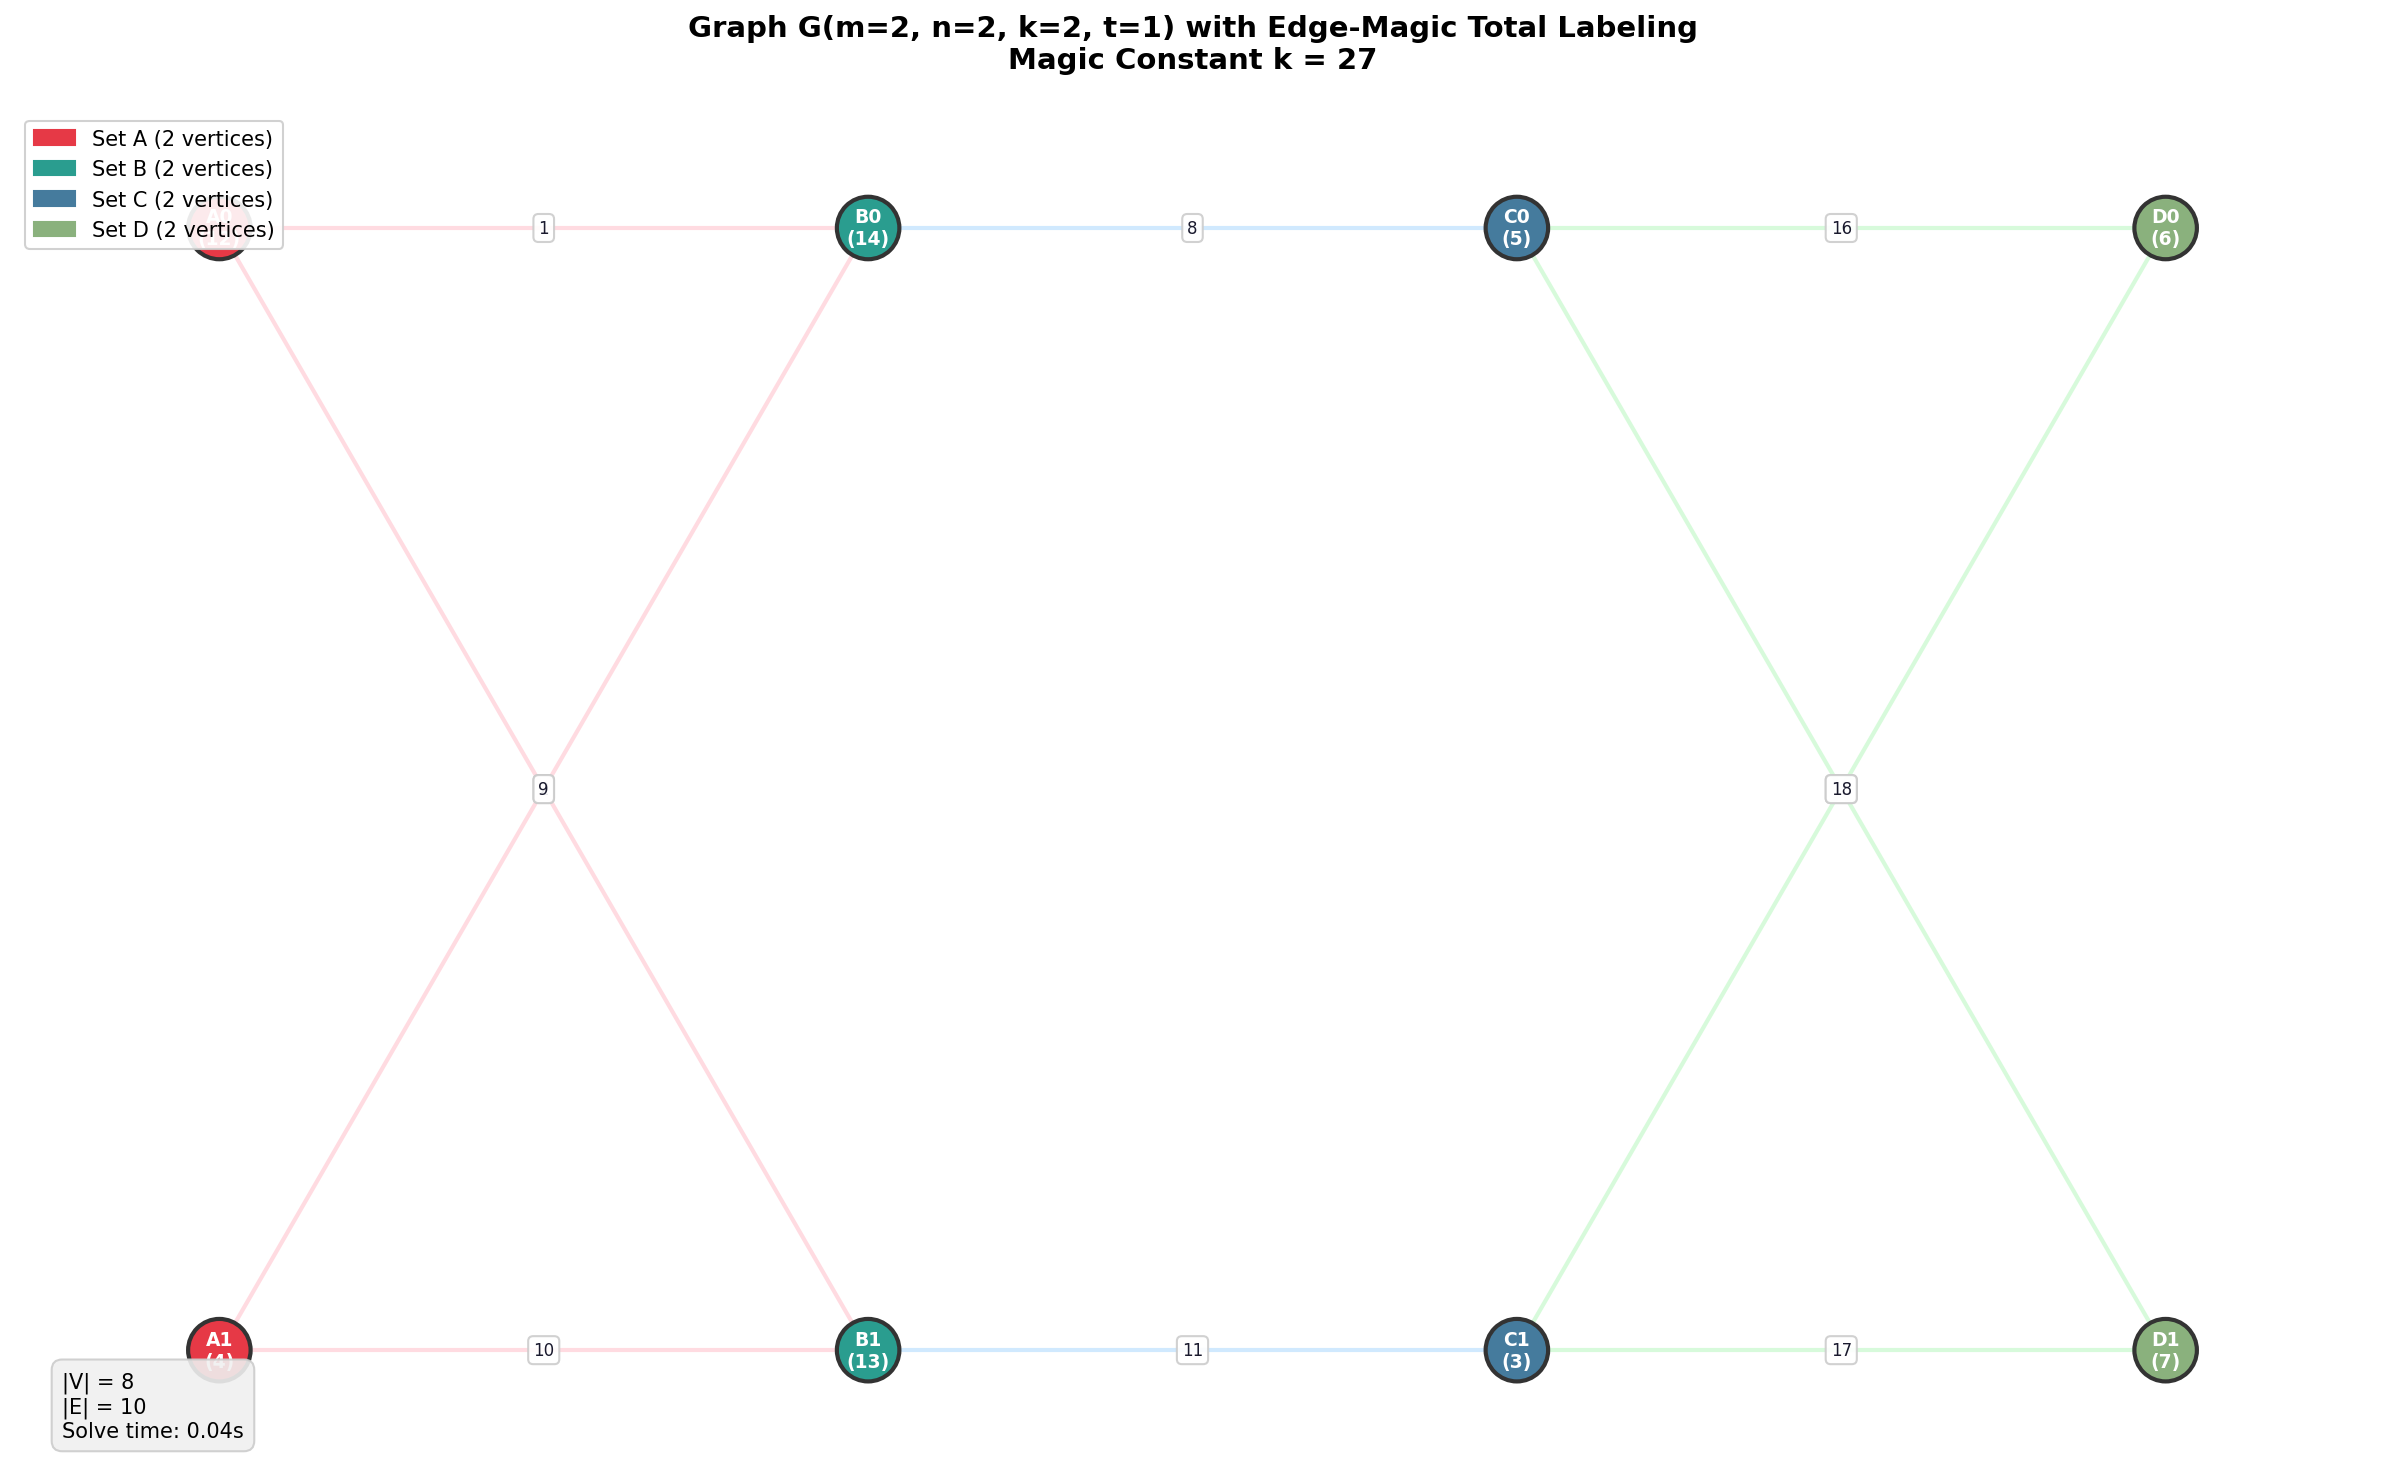
\includegraphics[width=0.82\textwidth]{emtl_m2_n2_k2_t1.png}
  \caption{The graph $G(2,2,2,1)$ with the four parts $A,B,C,D$ (left to right),
  the two complete-bipartite layers $K_{2,2}$ ($A$--$B$ and $C$--$D$) and the
  $1$-regular middle layer ($B$--$C$). Vertex and edge labels of a computed EMTL are
  shown; every edge sum equals the magic constant $\km$.}
  \label{fig:structure}
\end{figure}

\section{Algebraic necessary conditions}\label{sec:algebra}

This section records identities that every EMTL of $G$ must satisfy. They are not
needed to \emph{solve} an instance, but they constrain the magic constant, supply the
search bounds used by the solver, and act as independent post-solve checks.

Let $f$ be an EMTL of $G=(V,E)$ with magic constant $\km$. Summing the magic equation
of Definition~\ref{def:emtl} over all edges gives
\begin{equation}\label{eq:sum0}
  \sum_{uv\in E}\bigl(f(u)+f(uv)+f(v)\bigr) = |E|\,\km .
\end{equation}

\begin{lemma}[Endpoint sum as a degree-weighted vertex sum]\label{lem:endpoint}
$\displaystyle \sum_{uv\in E}\bigl(f(u)+f(v)\bigr)=\sum_{v\in V}\degr(v)\,f(v).$
\end{lemma}

\begin{proof}
Reorder the double sum by vertices: each label $f(v)$ is counted once for every edge
incident with $v$, of which there are $\degr(v)$, so
\[
  \sum_{uv\in E}\bigl(f(u)+f(v)\bigr)
   =\sum_{v\in V} f(v)\,\bigl|\{e\in E: v\in e\}\bigr|
   =\sum_{v\in V}\degr(v)\,f(v). \qedhere
\]
\end{proof}

\begin{proposition}[Degree-weighted identity]\label{prop:identity}
Let $S_N:=\sum_{i=1}^{N} i=\tfrac{N(N+1)}{2}$. Every EMTL of $G$ satisfies
\begin{equation}\label{eq:identity}
  |E|\,\km \;=\; S_N \;+\; \sum_{v\in V}\bigl(\degr(v)-1\bigr) f(v).
\end{equation}
\end{proposition}

\begin{proof}
Split~\eqref{eq:sum0} into edge- and vertex-contributions and apply
Lemma~\ref{lem:endpoint}:
\[
  |E|\,\km=\sum_{e\in E}f(e)+\sum_{v\in V}\degr(v)f(v).
\]
Because $f$ is a bijection onto $\{1,\dots,N\}$ we have
$\sum_{e\in E}f(e)+\sum_{v\in V}f(v)=S_N$, hence
$\sum_{e\in E}f(e)=S_N-\sum_{v\in V}f(v)$. Substituting yields~\eqref{eq:identity}.
\end{proof}

\begin{remark}
For $\Gfam$ the coefficient $\degr(v)-1$ takes only the values $n-1$ (on $A$ and $D$),
$m+t-1$ (on $B$), and $k+t-1$ (on $C$), by Proposition~\ref{prop:degrees}.
\end{remark}

\begin{corollary}[Divisibility / congruence condition]\label{cor:divis}
With the notation of Proposition~\ref{prop:identity},
\[
  \km=\frac{S_N+\sum_{v\in V}(\degr(v)-1)f(v)}{|E|},
  \qquad\text{so}\qquad
  S_N+\sum_{v\in V}(\degr(v)-1)f(v)\equiv 0 \pmod{|E|}.
\]
In particular, the numerator must be divisible by $|E|$. This is necessary but not
sufficient for an EMTL to exist.
\end{corollary}

\begin{proposition}[Universal bounds on the magic constant]\label{prop:bounds}
Every EMTL satisfies $\;6\le \km\le 3N-3$.
\end{proposition}

\begin{proof}
On an edge $uv$ the elements $u$, $uv$, $v$ are three distinct members of $V\cup E$,
so their labels are distinct because $f$ is injective. Any sum of three distinct labels
from $\{1,\dots,N\}$ is at least $1+2+3=6$ and at most $N+(N-1)+(N-2)=3N-3$; as this
holds for every edge, $\km$ obeys the same bounds. (Here $N=|V|+|E|\ge 3$ since $G$ has
at least one edge, so the range is nonempty.)
\end{proof}

The implementation uses Proposition~\ref{prop:bounds} as the domain of the
magic-constant variable in the constraint model of Section~\ref{sec:model}.

\section{Reduction and constraint model}\label{sec:model}

\subsection{The vertex-determination reduction}

The magic equation is functional in the edge label: rearranging
Definition~\ref{def:emtl} gives $f(uv)=\km-f(u)-f(v)$. This yields a clean reduction.

\begin{proposition}[Vertex-determination]\label{prop:reduction}
Let $G=(V,E)$ and fix a constant $\km$ and an injection $x\colon V\to\{1,\dots,N\}$.
Define the induced edge values $y_{uv}:=\km-x_u-x_v$ for $uv\in E$. Then $(\km,x)$
extends to an EMTL of $G$ if and only if
\begin{enumerate}[label=(\alph*),itemsep=1pt]
  \item $y_{uv}\in\{1,\dots,N\}$ for every $uv\in E$;
  \item the values $\{y_{uv}:uv\in E\}$ are pairwise distinct; and
  \item $\{y_{uv}:uv\in E\}\cap\{x_v:v\in V\}=\varnothing$.
\end{enumerate}
When these hold, the EMTL is unique given $(\km,x)$, namely $f|_V=x$ and $f(uv)=y_{uv}$.
\end{proposition}

\begin{proof}
If $f$ is an EMTL with $f|_V=x$ and magic constant $\km$, then the magic equation
forces $f(uv)=\km-x_u-x_v=y_{uv}$, so the edge labels are determined. Since $f$ is a
bijection onto $\{1,\dots,N\}$, every edge value satisfies $y_{uv}\in\{1,\dots,N\}$
(giving (a)), the $y_{uv}$ are pairwise distinct (giving (b)), and no $y_{uv}$ equals a
vertex label $x_v$ (giving (c)).
Conversely, if (a)--(c) hold, then $f$ defined by $f|_V=x$, $f(uv)=y_{uv}$ takes
values in $\{1,\dots,N\}$, is injective on $V\cup E$ (vertices are distinct by
hypothesis, edges by (b), and the two sets are disjoint by (c)), and therefore
bijective since $|V\cup E|=N$. By construction it satisfies every magic equation.
\end{proof}

Proposition~\ref{prop:reduction} shows that EMTL existence is, in principle, a search
over $\km$ and the vertex labeling alone: the edge labels never need to be guessed.
The solver below keeps explicit edge variables for clarity and for direct
verification, but it exploits exactly this structure --- fixing vertex labels forces
edge labels, which then propagates strongly through the bijection constraint.

\subsection{CP-SAT formulation}

We model EMTL existence as a constraint-satisfaction problem (no objective). Let
$N=|V|+|E|$.

\paragraph{Variables.}
\begin{itemize}[itemsep=1pt]
  \item a label variable $x_v\in\{1,\dots,N\}$ for each vertex $v\in V$;
  \item a label variable $x_e\in\{1,\dots,N\}$ for each edge $e\in E$ (written
        $x_{uv}$ when $e=uv$);
  \item the magic-constant variable $\km\in\{6,\dots,3N-3\}$
        (Proposition~\ref{prop:bounds}).
\end{itemize}

\paragraph{Constraints.}
\begin{align}
  &\AllDiff\bigl(\{x_v:v\in V\}\cup\{x_e:e\in E\}\bigr), \tag{C1}\label{eq:c1}\\
  &x_u+x_{uv}+x_v=\km \qquad\text{for every } uv\in E. \tag{C2}\label{eq:c2}
\end{align}
Since the $N$ label variables all share the domain $\{1,\dots,N\}$, constraint
\eqref{eq:c1} forces them to be a bijection onto $\{1,\dots,N\}$; \eqref{eq:c2} is the
magic property. The model therefore has $N+1$ integer variables, one all-different
constraint, and $|E|$ linear equations. By \eqref{eq:Vcount}--\eqref{eq:Ecount} the
model size can grow quadratically in the parameters --- the middle layer alone
contributes $nt$ edges, up to $n^2$ when $t=\Theta(n)$.

\subsection{Why CP-SAT}\label{sub:whycpsat}

We solve the model with Google OR-Tools CP-SAT~\cite{ortools}, a hybrid solver that
combines constraint propagation over integer domains with SAT-style
conflict-driven clause learning. Two features of the EMTL model make it a good fit.
First, by Proposition~\ref{prop:reduction} each magic equation~\eqref{eq:c2} is
functional, so as soon as two of the three labels on an edge are fixed the third is
forced; propagation thus turns partial vertex assignments into forced edge labels.
Second, the global all-different constraint~\eqref{eq:c1} couples every label, so a
single forced value can prune many domains, and learned conflict clauses prevent the
search from rediscovering the same infeasible patterns --- of which there are many,
since the family contains many structurally identical sub-configurations. When the
search exhausts the tree without a solution, the solver returns a genuine proof of
infeasibility rather than a mere timeout.

\section{Reference implementation}\label{sec:impl}

The solver is implemented in Python (\texttt{emtl\_solver.py}) on top of
\texttt{networkx} and OR-Tools, with a \texttt{matplotlib} visualizer and a Streamlit
web interface. Table~\ref{tab:impl} maps the mathematical objects of this paper to the
code. The end-to-end entry point \texttt{solve\_emtl(m,n,k,t,timeout)} validates the
parameters, constructs $\Gfam$, builds and solves the model of
Section~\ref{sec:model}, and independently verifies any returned labeling against
Definition~\ref{def:emtl}.

\begin{table}[t]
  \centering
  \small
  \begin{tabular}{@{}ll@{}}
    \toprule
    \textbf{Mathematical object} & \textbf{Code} \\
    \midrule
    Parameters $(m,n,k,t)$, counts $|V|,|E|,N$ & \texttt{GraphParameters} \\
    Graph $\Gfam$ and circulant layer~\eqref{eq:circulant} & \texttt{GraphConstructor.construct} \\
    Variables, \eqref{eq:c1}--\eqref{eq:c2}, solve & \texttt{EMTLSolver.solve} \\
    Bijection + magic check (Def.~\ref{def:emtl}) & \texttt{EMTLSolver.verify\_labeling} \\
    Drawing of a labeled instance & \texttt{EMTLVisualizer.visualize} \\
    Full pipeline & \texttt{solve\_emtl} \\
    \bottomrule
  \end{tabular}
  \caption{Correspondence between the formal model and the reference implementation.}
  \label{tab:impl}
\end{table}

\section{Experiments}\label{sec:experiments}

\paragraph{Setup.}
All runs use OR-Tools CP-SAT with the bounds of Proposition~\ref{prop:bounds}, a
per-instance time limit, and the solver's default portfolio of search workers.
Reported times are wall-clock seconds on a commodity laptop and are indicative
rather than benchmark-grade; the qualitative point is that small and moderate
instances of $\Gfam$ are decided quickly and exactly. For every instance reported as
\textsc{found}, the returned labeling was re-checked against
Definition~\ref{def:emtl} by an independent verifier; the \texttt{infeasible} verdict,
by contrast, is the solver's own unsatisfiability result and is not re-certified by an
external proof.

\paragraph{Results.}
Table~\ref{tab:results} summarizes representative runs; every instance was decided in
under half a second, and Figure~\ref{fig:examples} shows two of the computed labelings.

\begin{table}[t]
  \centering
  \small
  \begin{tabular}{@{}rrrrrrrlr@{}}
    \toprule
    $m$ & $n$ & $k$ & $t$ & $|V|$ & $|E|$ & $N$ & Outcome & Time (s) \\
    \midrule
    1 & 1 & 1 & 0 & 4  & 2  & 6  & infeasible (no EMTL) & 0.03 \\
    1 & 2 & 1 & 1 & 6  & 6  & 12 & $\km=17$ & 0.02 \\
    2 & 2 & 2 & 0 & 8  & 8  & 16 & $\km=26$ & 0.03 \\
    2 & 2 & 2 & 1 & 8  & 10 & 18 & $\km=27$ & 0.03 \\
    2 & 3 & 2 & 2 & 10 & 18 & 28 & $\km=33$ & 0.09 \\
    3 & 3 & 3 & 3 & 12 & 27 & 39 & $\km=50$ & 0.34 \\
    \bottomrule
  \end{tabular}
  \caption{Representative EMTL instances on $\Gfam$ with the magic constant found by
  CP-SAT (or a proof that none exists). Every labeling reported here was independently
  re-verified against Definition~\ref{def:emtl}.}
  \label{tab:results}
\end{table}

The smallest instance, $G(1,1,1,0)$, is \emph{infeasible}, and this is predicted by the
theory of Section~\ref{sec:algebra}: all four vertices have degree $1$, so every
coefficient $\degr(v)-1$ in~\eqref{eq:identity} vanishes and the identity reduces to
$|E|\,\km=S_N=21$ with $|E|=2$. Since $21$ is not divisible by $2$, Corollary~\ref{cor:divis}
already rules out any EMTL; the solver's infeasibility certificate matches this prediction.

\paragraph{A worked example.}
For $(m,n,k,t)=(2,2,2,1)$ we have $|V|=8$, $|E|=10$, and $N=18$.
The solver finds an EMTL with magic constant $\km=27$; one valid labeling is shown in
Figure~\ref{fig:structure}, and \texttt{verify\_labeling} confirms that all ten edge
sums equal $27$ and that the eighteen labels form a bijection onto $\{1,\dots,18\}$.

\begin{figure}[t]
  \centering
  \begin{minipage}{0.49\textwidth}
    \centering
    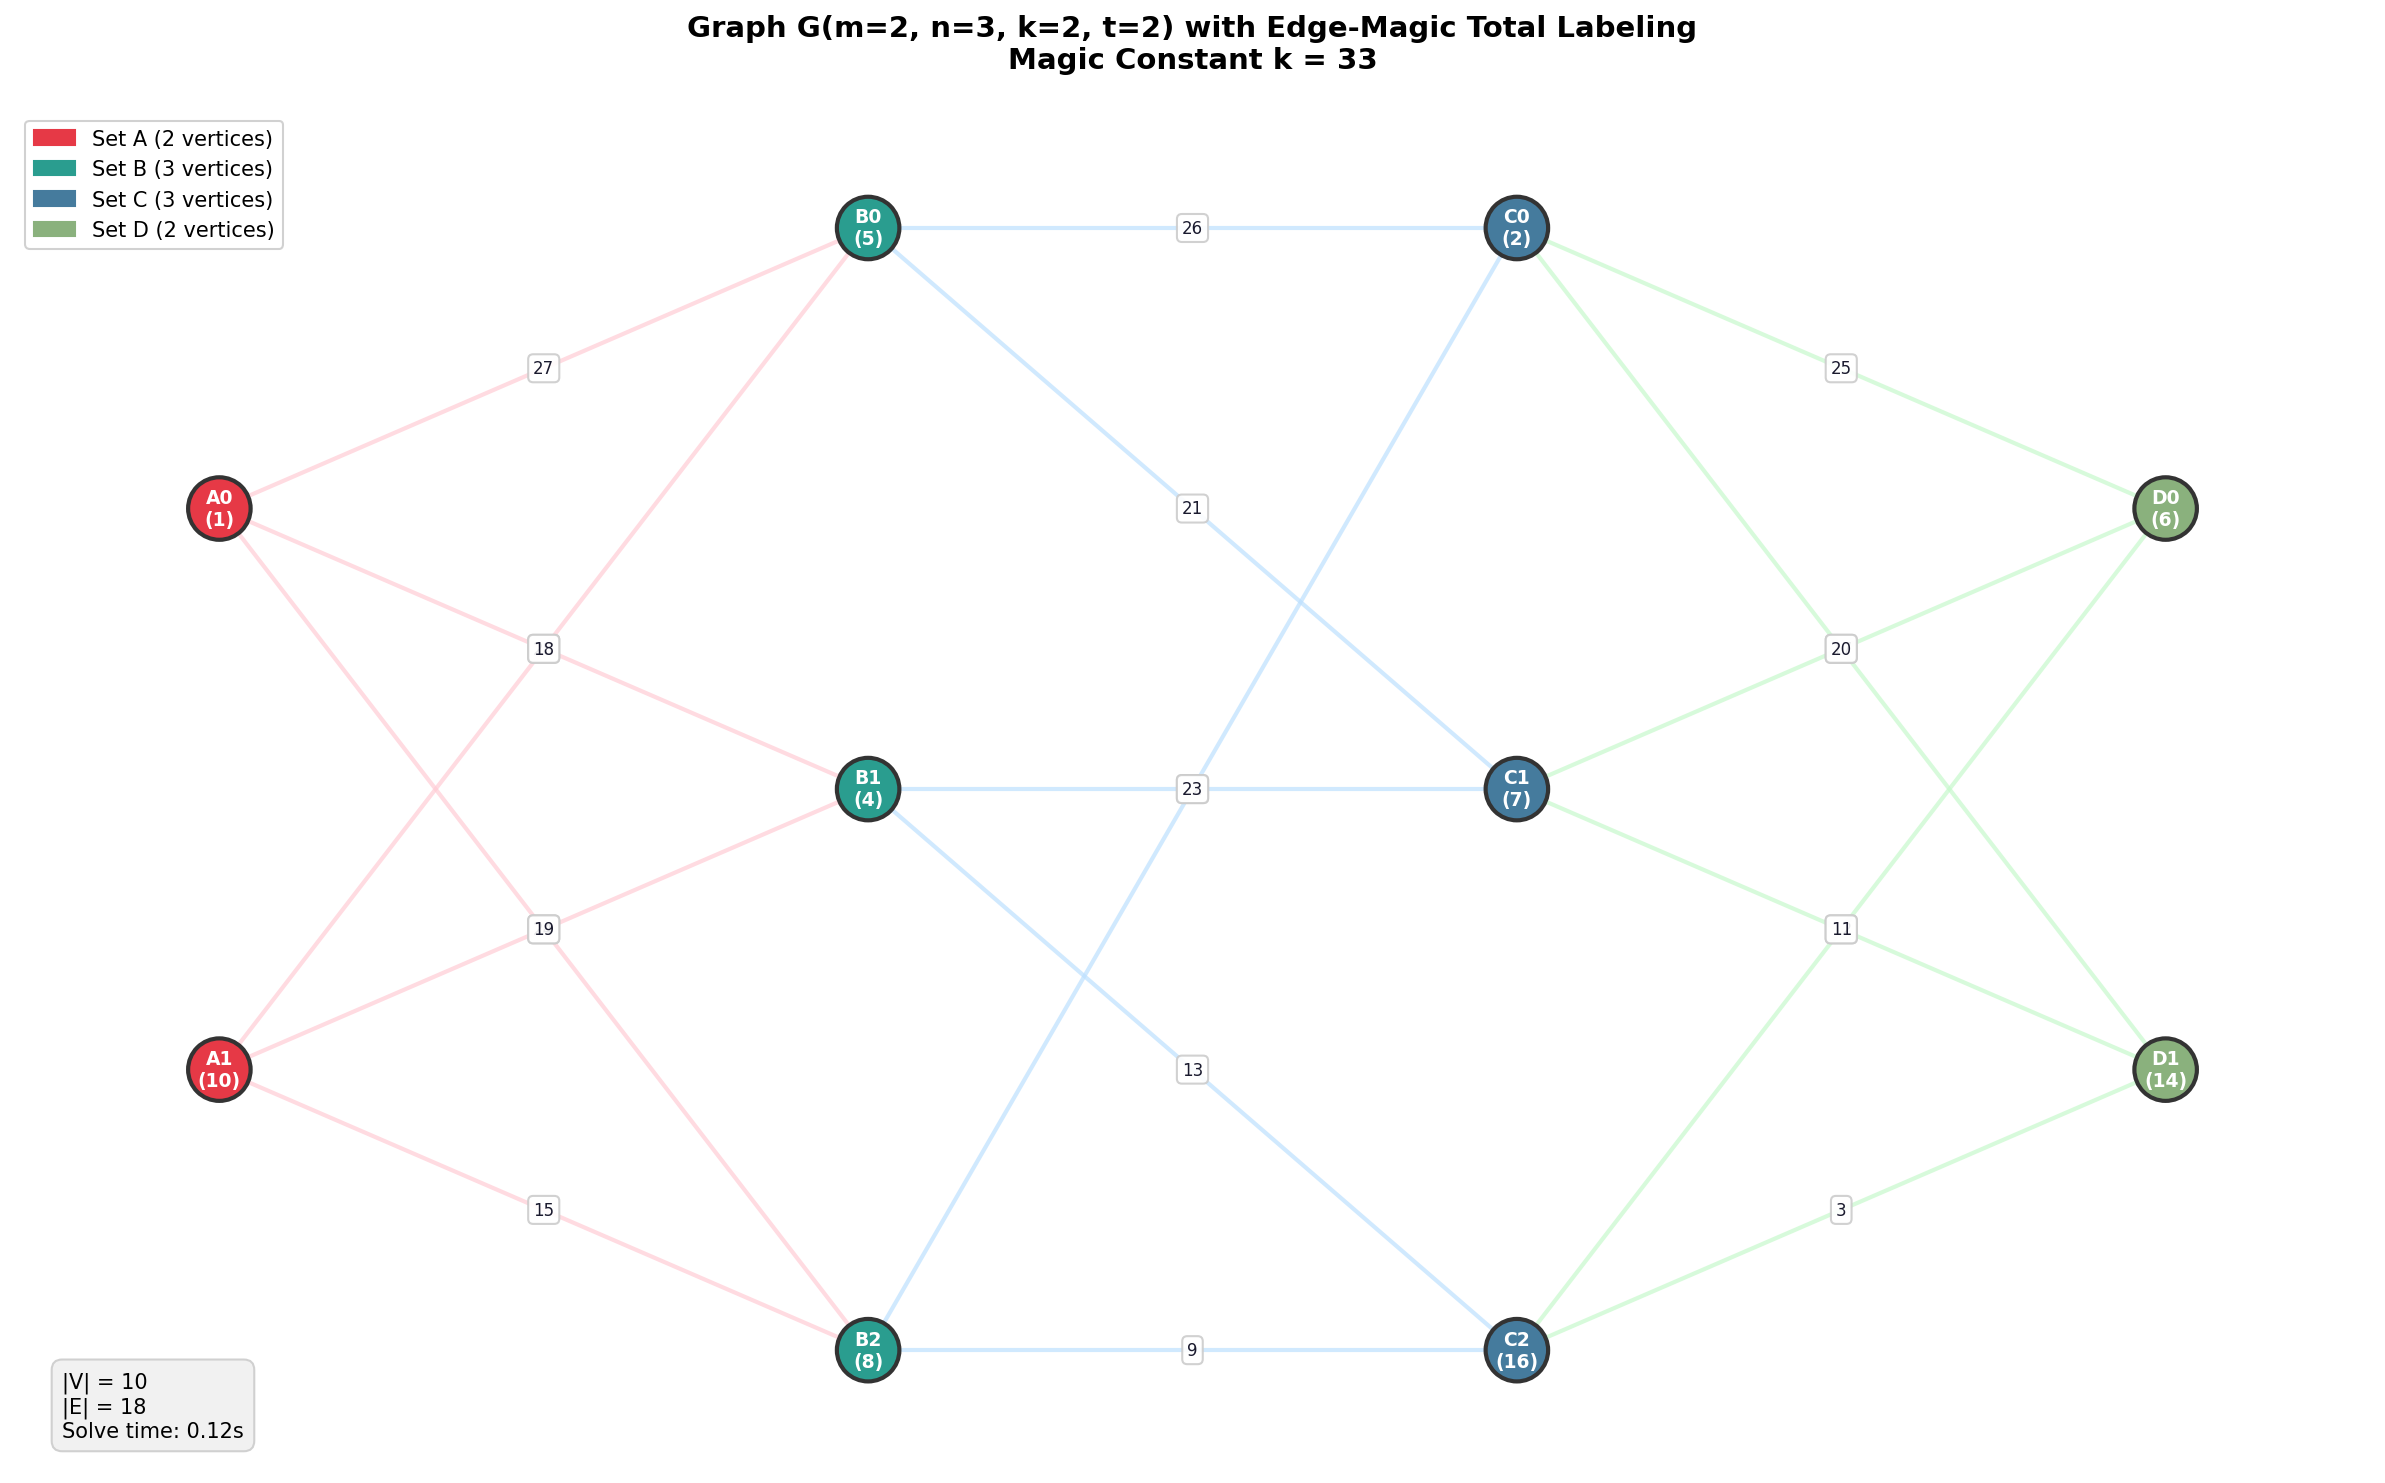
\includegraphics[width=\textwidth]{emtl_m2_n3_k2_t2.png}
    \subcaption{$G(2,3,2,2)$}
  \end{minipage}\hfill
  \begin{minipage}{0.49\textwidth}
    \centering
    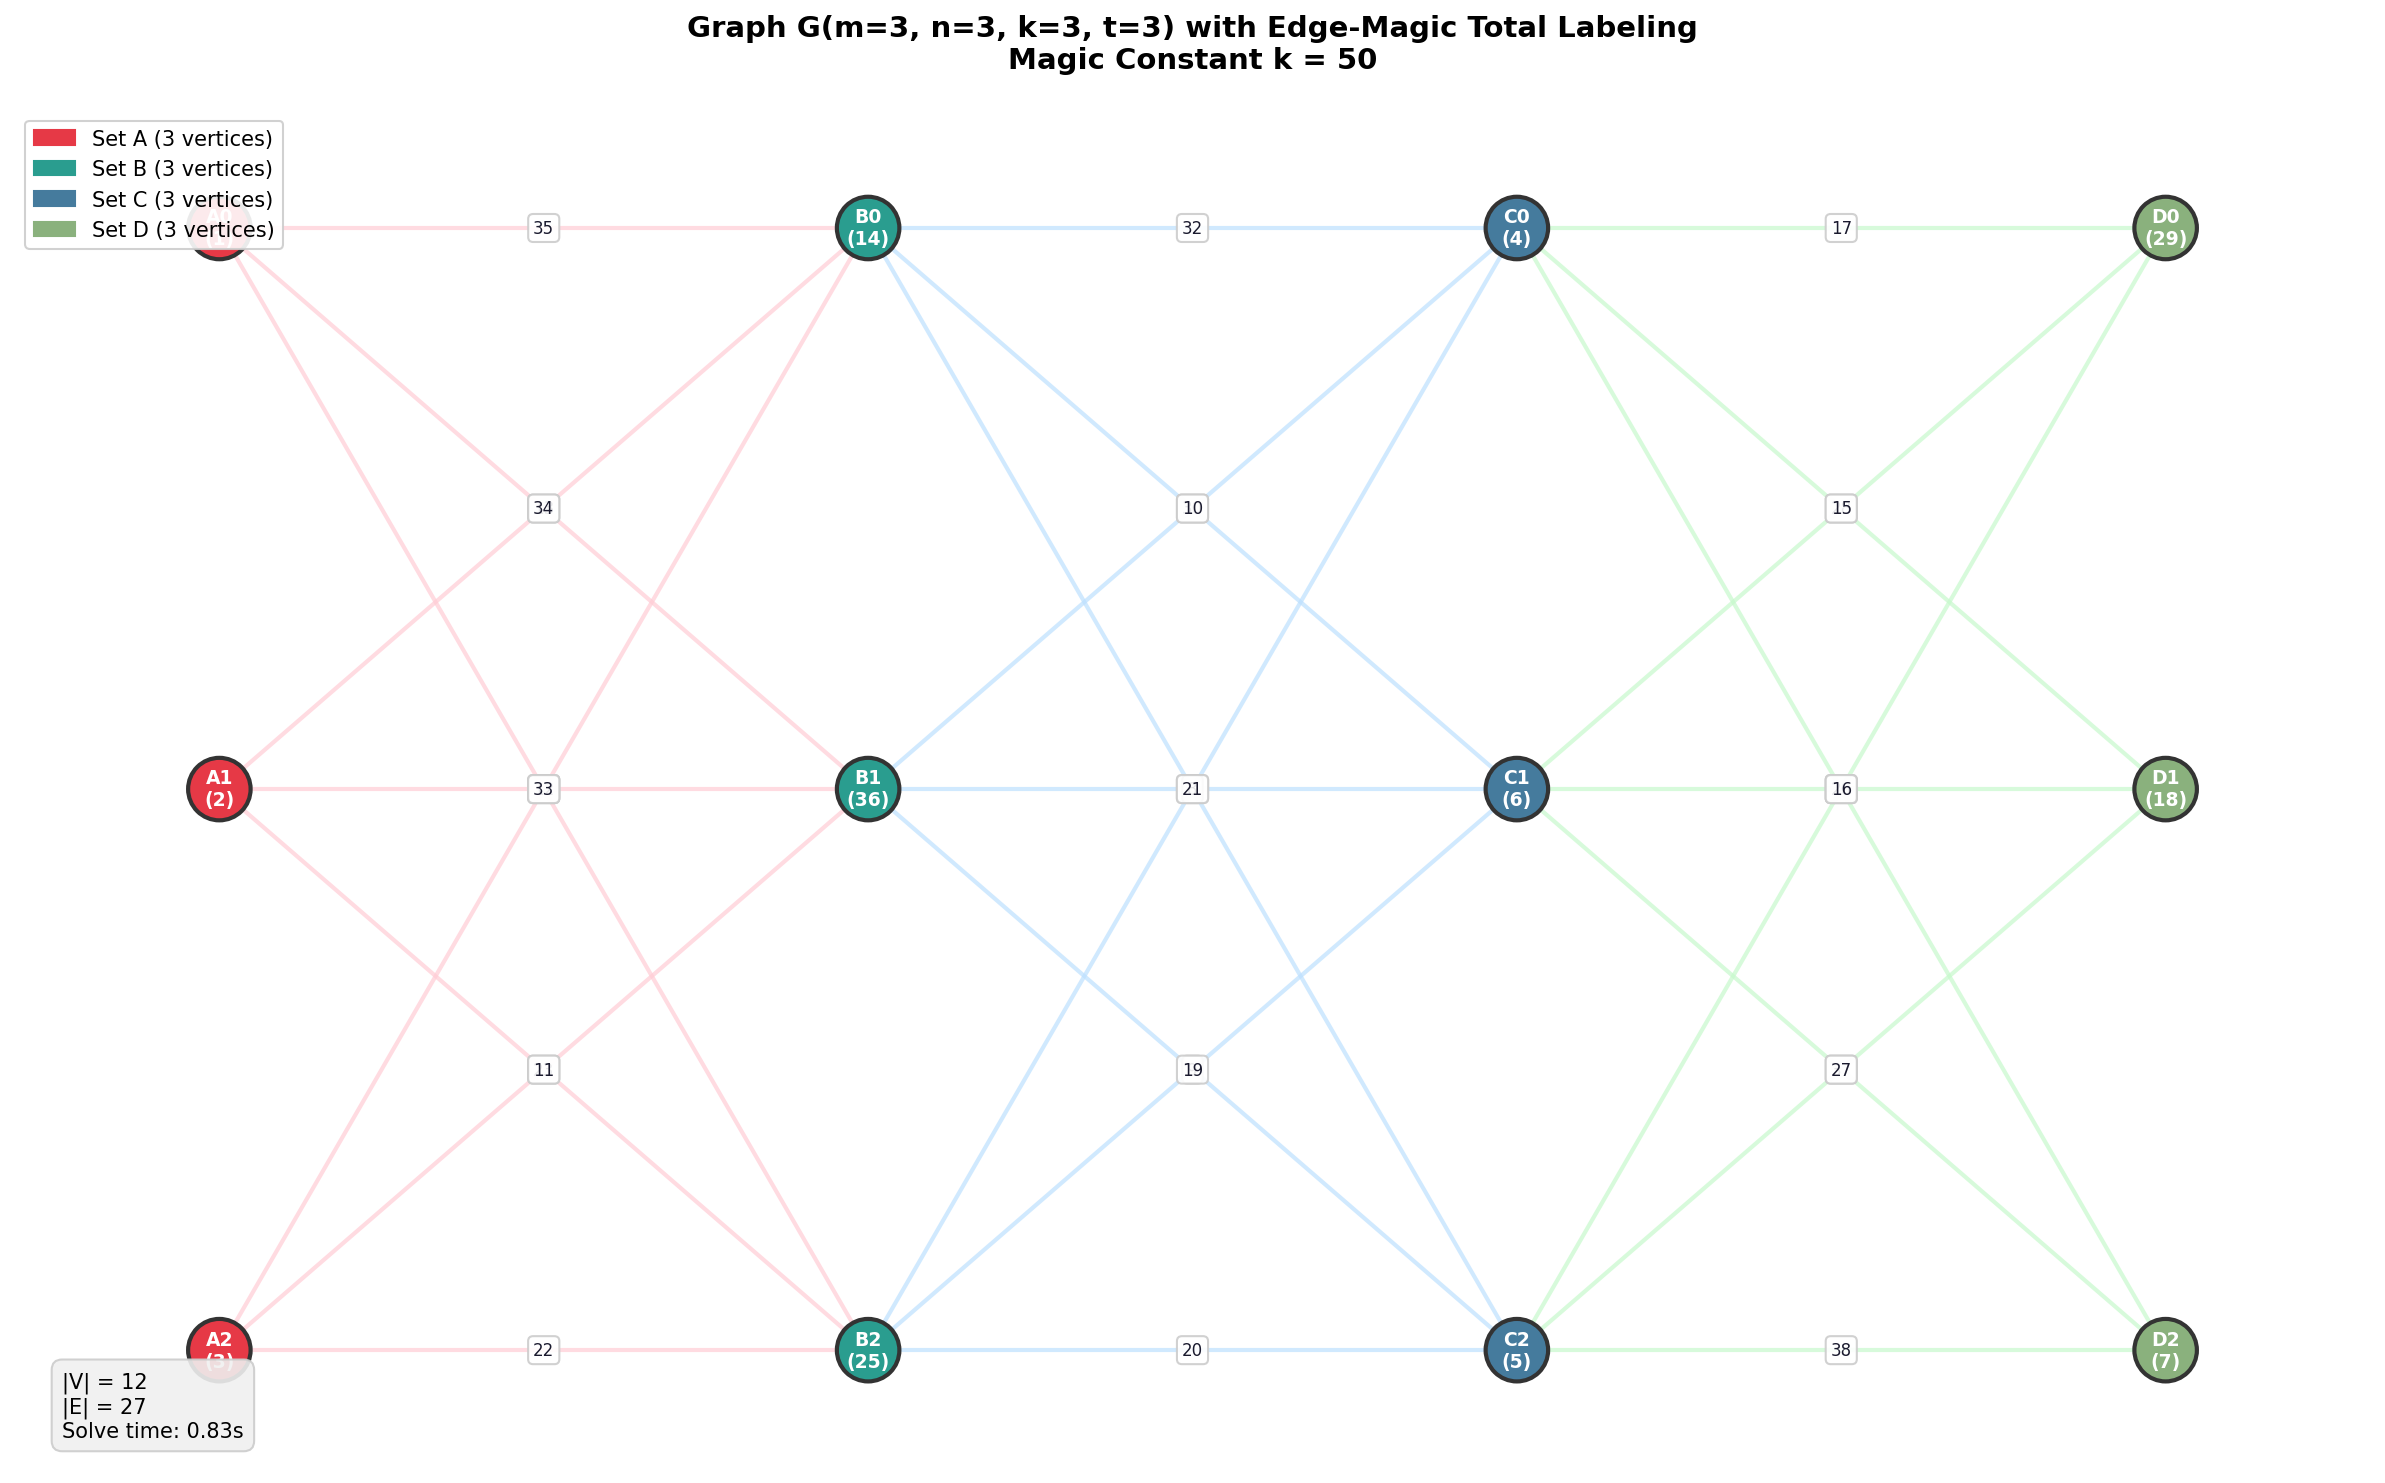
\includegraphics[width=\textwidth]{emtl_m3_n3_k3_t3.png}
    \subcaption{$G(3,3,3,3)$}
  \end{minipage}
  \caption{Computed edge-magic total labelings for two larger members of the family.
  Parts are colored $A,B,C,D$ from left to right; each edge label equals the magic
  constant minus its two endpoint labels.}
  \label{fig:examples}
\end{figure}

\section{Conclusion}\label{sec:conclusion}

We studied edge-magic total labelings on a structured four-partite family $\Gfam$. We
derived a degree-weighted identity, a divisibility condition, and bounds on the magic
constant, and proved a vertex-determination reduction that pins down the labeling once
the vertex labels and $\km$ are fixed. Casting existence as a constraint-satisfaction
problem and solving it with CP-SAT gives an exact method that returns a verified
labeling, an infeasibility proof, or a timeout. Natural next steps are to characterize
the parameter regions in which $\Gfam$ is edge-magic, to add symmetry-breaking
constraints exploiting the circulant structure of the middle layer, and to push the
solver to larger instances.

\paragraph{Availability.}
The source code, test suite, visualizer, and this article are available in the
project repository.

\begin{thebibliography}{9}
\bibitem{kotzig-rosa}
  A.~Kotzig and A.~Rosa,
  \emph{Magic valuations of finite graphs},
  Canad. Math. Bull. \textbf{13} (1970), 451--461.

\bibitem{wbms}
  W.~D.~Wallis, E.~T.~Baskoro, M.~Miller, and Slamin,
  \emph{Edge-magic total labelings},
  Australas. J. Combin. \textbf{22} (2000), 177--190.

\bibitem{wallis}
  W.~D.~Wallis,
  \emph{Magic Graphs},
  Birkh\"auser, Boston, 2001.

\bibitem{gallian}
  J.~A.~Gallian,
  \emph{A dynamic survey of graph labeling},
  Electron. J. Combin., Dynamic Survey \#DS6.

\bibitem{kite}
  I.~Singgih,
  \emph{Edge magic total labeling of $(n,t)$-kites},
  in Proc.\ Int.\ Conf.\ on Mathematics, Geometry, Statistics, and Computation
  (IC-MaGeStiC 2021), Atlantis Press, 2022, pp.\ 26--31.
  \url{https://www.atlantis-press.com/proceedings/ic-magestic-21/125970045}.

\bibitem{ortools}
  Google,
  \emph{OR-Tools CP-SAT solver} (documentation).
  \url{https://developers.google.com/optimization/cp/cp_solver}.
\end{thebibliography}

\end{document}
